%-------------------------------------------------------------------------------
%	EMPIEZA CAPITULO
%-------------------------------------------------------------------------------

\chapter{Criterio de Estabilidad de Routh-Hurwitz}

    \missingfigure{Diagrama de bloques de una función de transferencia general}

    Dado el sistema mostrado en la figura, tenemos que su función de transferencia es de la forma:

    \begin{equation}
        \frac{\hat{y}(s)}{\hat{r}(s)} = \frac{b_0 s^m + b_1 s^{m-1} + ... + b_{m-1} s + b_m}{a_0 s^n + a_1 s^{n-1} + ... + a_{n-1} s + a_n} = \frac{B(s)}{A(s)}
    \end{equation}

    es decir:

    \begin{equation}
        \frac{\hat{y}(s)}{\hat{r}(s)} = \sum{\frac{k_{1,i}}{s + \alpha_i}} + \sum{\frac{k_{2,j} + k_{3,j} \cdot s}{(s + \beta_i)^2 + {\gamma_i}^2}} ; m \leq n
    \end{equation}

    El criterio de Routh-Hurwitz determina si existen raíces en el semiplano complejo derecho cerrado.

%-------------------------------------------------------------------------------
%	EMPIEZA SECCION
%-------------------------------------------------------------------------------

    \newpage
    \section{Tabla de Routh}
        La tabla de Routh es un método para obtener el numero de raíces con parte real positiva que se encontraran en el polinomio característico del sistema (Ecuación~\ref{eqn:ECS}) sin tener que calcular las raíces en cuestión. Se puede dividir en cuatro pasos que se enumeran a continuación.

        \begin{equation} \label{eqn:ECS}
            A(s) = a_0 s^n + a_1 s^{n-1} + ... + a_{n-1} s + a_n = 0
        \end{equation}

        \begin{enumerate}
            \item Hipótesis
                Si $a_0 = 0 \Rightarrow$ el polinomio es de orden menor a $n$.

                Si $a_n = 0 \Rightarrow \exists$ una raíz que es $0 \Rightarrow A(s) = (\bar{n_0} s^{\bar{n}} + \bar{a_n} s^{\bar{n-1}} + ...) s^k $.

            \item Si existen coeficientes nulos o de diferente (cambio de) signo, entonces existen raíces con parte real positiva.
            \item Construir la tabla de Routh (Ver Cuadro~\ref{tab:Routh}).

            \begin{table}[htbp]
                \centering
                \begin{tabular}{c|c c c c c}
                    $s^n$     & $a_0$ & $a_2$ & $a_4$ & $a_6$ & ...\\
                    $s^{n-1}$ & $a_1$ & $a_3$ & $a_5$ & $a_7$ & ...\\
                    $s^{n-2}$ & $b_1$ & $b_3$ & $b_5$ & $b_7$ & ...\\
                    $s^{n-3}$ & $c_1$ & $c_3$ & $c_5$ & $c_7$ & ...\\
                    $s^{n-4}$ & $d_1$ & $d_3$ & $d_5$ & $d_7$ & ...\\
                    \vdots                                         \\
                    $s^2$ & $e_1$ & $e_2$                          \\
                    $s^1$ & $f_1$                                  \\
                    $s^0$ & $g_1$
                \end{tabular}
                \caption{\label{tab:Routh}Ejemplo de tabla de Routh.}
            \end{table}

            Donde:

            \begin{equation*}
            b_1 = \frac{a_1 a_2 - a_0 a_3}{a_1} , b_2 = \frac{a_1 a_4 - a_0 a_5}{a_1} , \dots
            \end{equation*}

            \begin{equation*}
            c_1 = \frac{b_1 a_3 - a_1 b_2}{b_1} , c_2 = \frac{b_1 a_5 - a_1 b_3}{b_1} , \dots
            \end{equation*}

            \begin{equation*}
            d_1 = \frac{c_1 b_2 - b_1 c_2}{c_1} , d_2 = \frac{c_1 b_3 - b_1 c_3}{c_1} , \dots
            \end{equation*}

            \begin{equation*}
            \vdots
            \end{equation*}

            \item El número de raíces con parte real positiva es igual al numero de cambios de signo en la primera columna(Ver Cuadro~\ref{tab:Numeros}).

            \begin{table}[htbp]
                \centering
                \begin{tabular}{c|c|}
                $s^n$     & $a_0$ \\
                $s^{n-1}$ & $a_1$ \\
                $s^{n-2}$ & $b_1$ \\
                $s^{n-3}$ & $c_1$ \\
                $s^{n-4}$ & $d_1$ \\
                \vdots & \vdots   \\
                $s^2$ & $e_1$     \\
                $s^1$ & $f_1$     \\
                $s^0$ & $g_1$
                \end{tabular}
            \caption{\label{tab:Numeros}Números en los que hay que revisar el cambio de signo.}
            \end{table}

        \end{enumerate}

%-------------------------------------------------------------------------------
%	EMPIEZA SECCION
%-------------------------------------------------------------------------------

    \newpage
    \section{Casos Especiales}
        \begin{enumerate}

            \item En los casos en los que un coeficiente es $0$ se puede intercambiar por un $\epsilon$ lo suficientemente pequeño para aproximar a $0$ (Véase el Cuadro~\ref{tab:Caso1}).

            \begin{equation*}
            A(s) = s^3 + 2 s^2 + s + 2 = 0
            \end{equation*}

            \begin{verbatim}
            >> A = [1 2 1 2];
            >> r = roots(A)
            r =
              -2.00000 + 0.00000i
              -0.00000 + 1.00000i
              -0.00000 - 1.00000i
            \end{verbatim}

            \begin{table}[htbp]
                \centering
                \begin{tabular}{c|c c}
                $s^3$ & $1$ & $1$ \\
                $s^2$ & $2$ & $2$ \\
                $s^1$ & $0 \approx \epsilon$ \\
                $s^0$ & $2$
                \end{tabular}
            \caption{\label{tab:Caso1}Caso Especial 1.}
            \end{table}

            \item Cuando existen cambios en los coeficientes del polinomio característico se sabe que existirán raíces con parte real positiva (Véase el Cuadro~\ref{tab:Caso2}).

            \begin{equation*}
                A(s) = s^3 - 3 s + 2 = 0
            \end{equation*}

            \begin{verbatim}
            >> A = [1 0 -3 2];
            >> r = roots(A)
            r =
              -2.00000
               1.00000
               1.00000
            \end{verbatim}

            \begin{table}[htbp]
                \centering
                \begin{tabular}{c|c c}
                $s^3$ & $1$ & $-3$ \\
                $s^2$ & $0\approx\epsilon$ & $2$ \\
                $s^1$ & $-\frac{2}{\epsilon}$ & $0$ \\
                $s^0$ & $2$
                \end{tabular}
                \caption{\label{tab:Caso2}Caso Especial 2.}
            \end{table}

            \item Cuando todos los coeficientes en una linea se eliminan se puede crear un nuevo polinomio auxiliar con la linea anterior, obtener su derivada e insertar en la siguiente linea para continuar calculando la tabla (Véase el Cuadro~\ref{tab:Caso3a} y~\ref{tab:Caso3b}).

            \begin{equation*}
            A(s) = s^5 + 2 s^4 + 24 s^3 + 48 s^2 - 25 s - 50 = 0
            \end{equation*}

            \begin{equation*}
            p_{aux}(s) = 2 s^4 + 48 s^2 - 50
            \end{equation*}

            \begin{equation*}
            \frac{d}{d x} p_{aux}(s) = 8 s^3 + 96 s
            \end{equation*}

            \begin{verbatim}
            >> A = [1 2 24 48 -25 -50];
            >> r = roots(A)
            r =
              -0.00000 + 5.00000i
              -0.00000 - 5.00000i
               1.00000 + 0.00000i
              -2.00000 + 0.00000i
              -1.00000 + 0.00000i
            \end{verbatim}

            \begin{table}[htbp]
                \centering
                \begin{tabular}{c|c c c}
                $s^5$ & $1$ & $24$ & $-25$ \\
                $s^4$ & $2$ & $48$ & $-50$ \\
                $s^3$ & $0$ & $0$  & $0$   \\
                $s^2$ \\
                $s^1$ \\
                $s^0$
                \end{tabular}
                \caption{\label{tab:Caso3a}Caso Especial 3a.}
            \end{table}

            \begin{table}[htbp]
                \centering
                \begin{tabular}{c|c c c}
                $s^5$ & $1$ & $24$ & $-25$ \\
                $s^4$ & $2$ & $48$ & $-50$ \\
                $s^3$ & $8$ & $96$ & $0$   \\
                $s^2$ & $24$ & $-50$ & $0$ \\
                $s^1$ & $112.6$ & $0$ \\
                $s^0$ & $-50$
                \end{tabular}
                \caption{\label{tab:Caso3b}Caso Especial 3b.}
            \end{table}

        \end{enumerate}

        \begin{figure*}
            \centering
            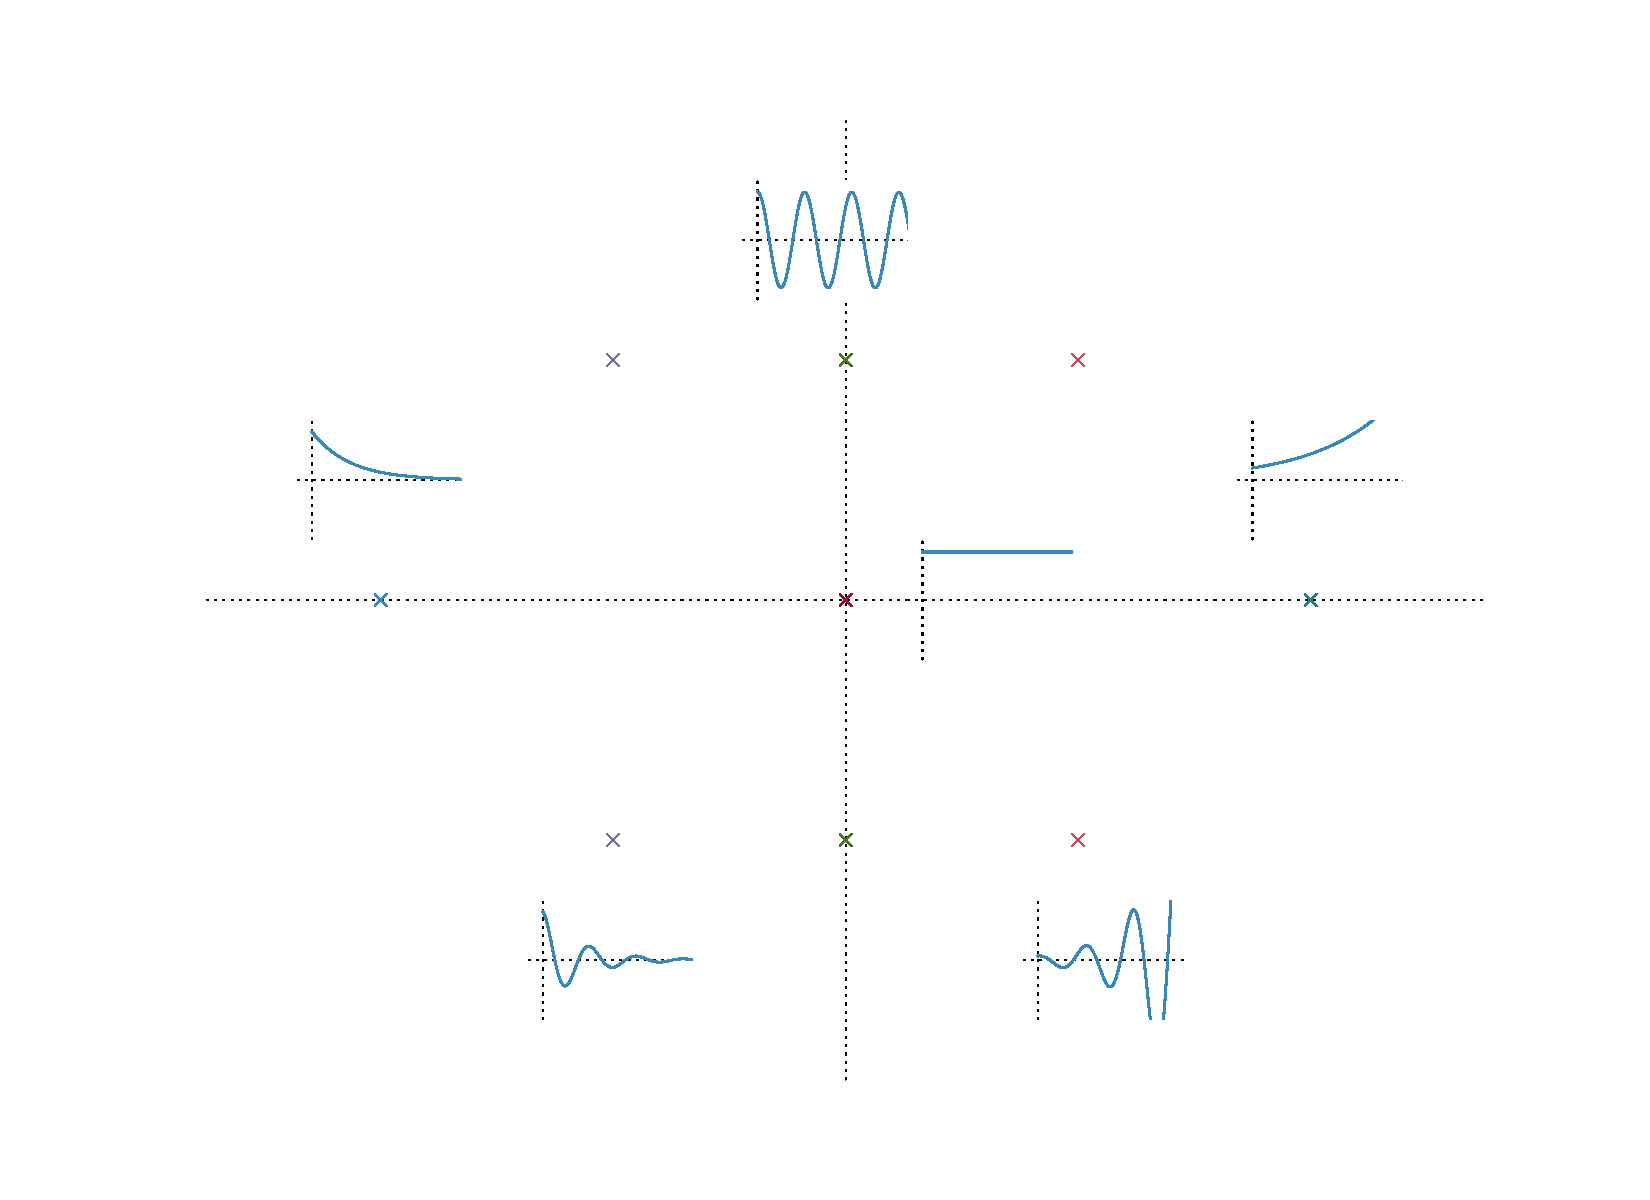
\includegraphics[width=0.9\textwidth]{./imagenes/planocomplejo.pdf}
            \caption{\label{fig:planocomplejo}Polos en el plano complejo.}
        \end{figure*}

%-------------------------------------------------------------------------------
%	EMPIEZA SECCION
%-------------------------------------------------------------------------------

    \newpage
    \section{Aplicación del criterio de Routh}
        Si bien los sistemas numéricos actuales permiten el calculo de las raíces de un sistema de manera mas rápida y sencilla que con la aplicación de este método, aun existen aplicaciones practicas en las que es de suma importancia el determinar el numero de raíces positivas. Por ejemplo podemos tener ganancias en un sistema para las que queremos determinar de primera instancia, un rango de valores para los cuales el sistema no se volverá inestable.

        Para ello calculamos la tabla de Routh de la misma manera en que lo hicimos anteriormente, pero teniendo en cuenta las ganancias a incluir en el calculo de las raíces (Por ejemplo con una ganancia proporcional véase Cuadro~\ref{tab:Aplicacion}).

        \begin{table}[htbp]
            \centering
            \begin{tabular}{c|c c c c c}
            $s^n$     & $a_0$ & $a_2$ & $a_4$ & $a_6$ & ...\\
            $s^{n-1}$ & $a_1$ & $a_3$ & $a_5$ & $a_7$ & $k$\\
            $s^{n-2}$ & $b_1$ & $b_3$ & $b_5$ & $b_7$ & ...\\
            $s^{n-3}$ & $c_1$ & $c_3$ & $c_5$ & $c_7$ & ...\\
            $s^{n-4}$ & $d_1$ & $d_3$ & $d_5$ & $d_7$ & ...\\
            \vdots                                         \\
            $s^2$ & $e_1$ & $e_2$                          \\
            $s^1$ & $f_1$                                  \\
            $s^0$ & $g_1$
            \end{tabular}
            \caption{\label{tab:Aplicacion}Aplicación del criterio de Routh.}
        \end{table}

%-------------------------------------------------------------------------------

        \subsection{Ejemplo}

            \begin{figure}
                \centering
                \resizebox{0.7\textwidth}{!}{
                    \tikzstyle{block} = [draw, rectangle, minimum height=3em, minimum width=4em]
                    \tikzstyle{sum} = [draw, circle]

                    \begin{tikzpicture}[auto, node distance=2cm, >=latex']
                        \node [input, name=entrada] {};
                        \node [sum, right of=entrada] (suma) {$+$};
                        \node [block, right of=suma] (planta) {$\frac{k}{s(s^2 + s + 4)(s+2)}$};
                        \node [output, right of=planta] (salida) {};
                        \node [block, below of=planta] (retro) {$-1$};

                        \draw [->] (entrada) -- node[name=u] {$\hat{r}(s)$} (suma);
                        \draw [->] (suma) -- (planta);
                        \draw [->] (planta) -- node[name=y] {$\hat{y}(s)$} (salida);
                        \draw [->] (y) |- (retro);
                        \draw [->] (retro) -| (suma);
                    \end{tikzpicture}}
                \caption{\label{dia:est1}Sistema para analizar estabilidad por el criterio de Routh - Hurwitz.}
            \end{figure}

            Se toma el sistema $\frac{\hat{y}(s)}{\hat{r}(s)} = \frac{k}{s^4 + 3 s^3 + 3 s^2 + 2 s + k}$, entonces el polinomio característico del sistema será $F(s) = s^4 + 3 s^3 + 3 s^2 + 2 s + k$.

            Construimos su tabla de Routh (Cuadro~\ref{tab:EjemploAplicacion}):

            \begin{table}[htbp]
                \centering
                \begin{tabular}{c|c c c}
                $s^4$ & $1$ & $3$ & $k$ \\
                $s^3$ & $3$ & $2$ & $0$ \\
                $s^2$ & $\sfrac{7}{3}$ & $k$ & $0$ \\
                $s^1$ & $2 - \sfrac{9}{7} k$ & $0$ \\
                $s^0$ & $k$
                \end{tabular}
                \caption{\label{tab:EjemploAplicacion}Ejemplo de Aplicación del criterio de Routh.}
            \end{table}

            De lo anterior podemos concluir que, para que no existan cambios de signos, toda la primera columna tiene que ser positiva, por lo que $k > 0$ y  $2 - \sfrac{9}{7} k > 0$, por lo que el rango de valores que puede ocupar la ganancia $k$ es $0 < k < \sfrac{14}{9}$

            Si bien esto no nos aporta una ganancia especifica para un comportamiento deseado, si nos da la pauta a los valores a tomar en cuenta, si no se desea que el sistema sea inestable.

%-------------------------------------------------------------------------------
%	EMPIEZA SECCION
%-------------------------------------------------------------------------------

    \newpage
    \section{Acción Proporcional}

        \begin{figure}
            \centering
            \resizebox{0.7\textwidth}{!}{
                \tikzstyle{block} = [draw, rectangle, minimum height=3em, minimum width=4em]
                \tikzstyle{sum} = [draw, circle]

                \begin{tikzpicture}[auto, node distance=2cm, >=latex']
                    \node [input, name=entrada] {};
                    \node [sum, right of=entrada] (suma) {$+$};
                    \node [block, right of=suma] (ganancia) {$k$};
                    \node [block, right of=ganancia] (planta) {$\frac{1}{Ts + 1}$};
                    \node [output, right of=planta] (salida) {};
                    \node [block, below of=planta] (retro) {$-1$};

                    \draw [->] (entrada) -- node[name=x] {$\hat{r}(s)$} (suma);
                    \draw [->] (suma) -- node[name=e] {$e$} (ganancia);
                    \draw [->] (ganancia) -- node[name=u] {$u$} (planta);
                    \draw [->] (planta) -- node[name=y] {$\hat{y}(s)$} (salida);
                    \draw [->] (y) |- (retro);
                    \draw [->] (retro) -| (suma);
                \end{tikzpicture}}
            \caption{\label{dia:est2}Sistema de primer orden con controlador proporcional.}
        \end{figure}

        Tenemos un sistema de primer orden, al que le agregaremos un controlador de ganancia proporcional y una retroalimentación negativa, por lo que las ecuaciones que describen la salida y el error del sistema quedan:

    \begin{equation}
        \frac{\hat{y}(s)}{\hat{r}(s)} = \frac{k}{Ts + 1 + k}
    \end{equation}

    \begin{equation}
        \frac{\hat{e}(s)}{\hat{r}(s)} = \frac{\hat{r}(s) - \hat{y}(s)}{\hat{r}(s)} = \frac{Ts + 1}{Ts + 1 + k}
    \end{equation}

        \subsection{Estabilidad}
            El problema reside en encontrar un conjunto de ganancias $k$ para las cuales el sistema es estable.
            \begin{equation}
                F(s) = s + \frac{1 + k}{T}
            \end{equation}

            Aplicamos una tabla de Routh a este polinomio característico (Cuadro~\ref{tab:AccionProporcional}).

            \begin{table}[htbp]
                \centering
                \begin{tabular}{c|c}
                $s^1$ & $1$ \\
                $s^0$ & $\sfrac{1+k}{T}$
                \end{tabular}
                \caption{\label{tab:AccionProporcional}Tabla de Routh para acción proporcional.}
            \end{table}

Por lo que concluimos que la ganancia $k$ debe de seguir: $k>-1$

%-------------------------------------------------------------------------------

        \subsection{Error en el estado permanente al escalón unitario}
            También es importante investigar el error que causara el controlador al introducirse. Si ponemos como señal de referencia al escalón unitario($R(s) = \frac{1}{s}$), podemos ver lo siguiente:

            \begin{equation*}
                \displaystyle \lim_{t \to \infty} e(t) = \lim_{s \to 0} s e(s) = \lim_{s \to 0} \frac{Ts + 1}{Ts + 1 + k} = \frac{1}{1 + k}
            \end{equation*}

            \missingfigure{Gráfica de respuesta sobreamortiguada y con error en estado estacionario.}

%-------------------------------------------------------------------------------
%	EMPIEZA SECCION
%-------------------------------------------------------------------------------

    \newpage
    \section{Acción Integral}

        \begin{figure}
            \centering
            \resizebox{0.7\textwidth}{!}{
                \tikzstyle{block} = [draw, rectangle, minimum height=3em, minimum width=4em]
                \tikzstyle{sum} = [draw, circle]

                \begin{tikzpicture}[auto, node distance=2cm, >=latex']
                    \node [input, name=entrada] {};
                    \node [sum, right of=entrada] (suma) {$+$};
                    \node [block, right of=suma] (ganancia) {$\frac{k}{s}$};
                    \node [block, right of=ganancia] (planta) {$\frac{1}{Ts + 1}$};
                    \node [output, right of=planta] (salida) {};
                    \node [block, below of=planta] (retro) {$-1$};

                    \draw [->] (entrada) -- node[name=x] {$\hat{r}(s)$} (suma);
                    \draw [->] (suma) -- node[name=e] {$e$} (ganancia);
                    \draw [->] (ganancia) -- node[name=u] {$u$} (planta);
                    \draw [->] (planta) -- node[name=y] {$\hat{y}(s)$} (salida);
                    \draw [->] (y) |- (retro);
                    \draw [->] (retro) -| (suma);
                \end{tikzpicture}}
            \caption{\label{dia:est3}Sistema de primer orden con controlador integral.}
        \end{figure}

        Tenemos un sistema de primer orden, al que le agregaremos un controlador de ganancia integral y una realimentación negativa, por lo que las ecuaciones que describen la salida y el error del sistema quedan:

        \begin{equation}
            \frac{\hat{y}(s)}{\hat{r}(s)} = \frac{k}{s(Ts + 1) + k}
        \end{equation}

        \begin{equation}
            \frac{\hat{e}(s)}{\hat{r}(s)} = \frac{\hat{r}(s) - \hat{y}(s)}{\hat{r}(s)} = \frac{s(Ts + 1)}{s(Ts + 1) + k}
        \end{equation}

%-------------------------------------------------------------------------------

        \subsection{Estabilidad}
            El problema reside en encontrar un conjunto de ganancias $k$ para las cuales el sistema es estable.
            \begin{equation}
                F(s) = s^2 + \frac{1}{T} s + \frac{k}{T}
            \end{equation}

            Aplicamos una tabla de Routh a este polinomio característico (Cuadro~\ref{tab:AccionIntegral}).

            \begin{table}[htbp]
                \centering
                \begin{tabular}{c|c c}
                $s^2$ & $1$ & $\sfrac{k}{T}$ \\
                $s^1$ & $\sfrac{1}{T}$ & $0$ \\
                $s^0$ & $\sfrac{k}{T}$
                \end{tabular}
                \caption{\label{tab:AccionIntegral}Tabla de Routh para acción integral.}
            \end{table}

            Por lo que concluimos que la ganancia $k$ debe de seguir: $k>0$

%-------------------------------------------------------------------------------

        \subsection{Error en el estado permanente al escalón unitario}
            También es importante investigar el error que causará el controlador al introducirse. Si ponemos como señal de referencia al escalón unitario($\hat{r}(s) = \frac{1}{s}$), podemos ver lo siguiente:

            \begin{equation*}
                \displaystyle \lim_{t \to \infty} e(t) = \lim_{s \to 0} s e(s) = \lim_{s \to 0} s \left(\frac{s(Ts + 1)}{s(Ts + 1) + k} \frac{1}{s}\right) = 0
            \end{equation*}

            \begin{figure}
                \centering
                \resizebox{0.7\textwidth}{!}{
                    \tikzstyle{block} = [draw, rectangle, minimum height=3em, minimum width=4em]
                    \tikzstyle{sum} = [draw, circle]

                    \begin{tikzpicture}[auto, node distance=2cm, >=latex']
                        \node [input, name=entrada] {};
                        \node [sum, right of=entrada] (suma) {$+$};
                        \node [block, right of=suma] (ganancia) {$\frac{k}{s}$};
                        \node [block, right of=ganancia] (planta) {$\frac{1}{s(Js + b)}$};
                        \node [output, right of=planta] (salida) {};
                        \node [block, below of=planta] (retro) {$-1$};

                        \draw [->] (entrada) -- node[name=x] {$\hat{r}(s)$} (suma);
                        \draw [->] (suma) -- node[name=e] {$e$} (ganancia);
                        \draw [->] (ganancia) -- node[name=u] {$u$} (planta);
                        \draw [->] (planta) -- node[name=y] {$\hat{y}(s)$} (salida);
                        \draw [->] (y) |- (retro);
                        \draw [->] (retro) -| (suma);
                    \end{tikzpicture}}
                \caption{\label{dia:est2}Sistema de segundo orden con controlador proporcional.}
            \end{figure}

            \faltante{Falta escribir apunte}

%-------------------------------------------------------------------------------
%	EMPIEZA SECCION
%-------------------------------------------------------------------------------

    \newpage
    \section{Acción Proporcional Integral}

        \begin{figure}
            \centering
            \resizebox{0.7\textwidth}{!}{
                \tikzstyle{block} = [draw, rectangle, minimum height=3em, minimum width=4em]
                \tikzstyle{sum} = [draw, circle]

                \begin{tikzpicture}[auto, node distance=2cm, >=latex']
                    \node [input, name=entrada] {};
                    \node [sum, right of=entrada] (suma1) {$+$};
                    \node [block, right of=suma1] (ganancia) {$k_p\left( 1 + \frac{1}{T_i s} \right)$};
                    \node [sum, right of=ganancia, pin={[init]above:$d$}] (suma2) {$+$};
                    \node [block, right of=suma2] (planta) {$\frac{1}{s(Js + b)}$};
                    \node [output, right of=planta] (salida) {};
                    \node [block, below of=planta] (retro) {$-1$};

                    \draw [->] (entrada) -- node[name=x] {$\hat{r}(s)$} (suma1);
                    \draw [->] (suma1) -- node[name=e] {$e$} (ganancia);
                    \draw [->] (ganancia) -- node[name=u] {$u$} (suma2);
                    \draw [->] (suma2) -- (planta);
                    \draw [->] (planta) -- node[name=y] {$\hat{y}(s)$} (salida);
                    \draw [->] (y) |- (retro);
                    \draw [->] (retro) -| (suma);
                \end{tikzpicture}}
            \caption{\label{dia:est4}Sistema de segundo orden con controlador proporcional integral.}
        \end{figure}

        \faltante{Falta escribir apunte}

%-------------------------------------------------------------------------------

        \subsection{Estabilidad}
        \faltante{Falta escribir apunte}

%-------------------------------------------------------------------------------

        \subsection{Error en el estado permanente al escalón unitario}
        \faltante{Falta escribir apunte}
